\chapter{Public Transport}
\label{ch:pt}
% ##################################################################################################################

\hfill \textbf{Authors:} Marcel Rieser, Andreas Neumann, Johan W. Joubert, Sergio Arturo Ordóñez

\begin{center} 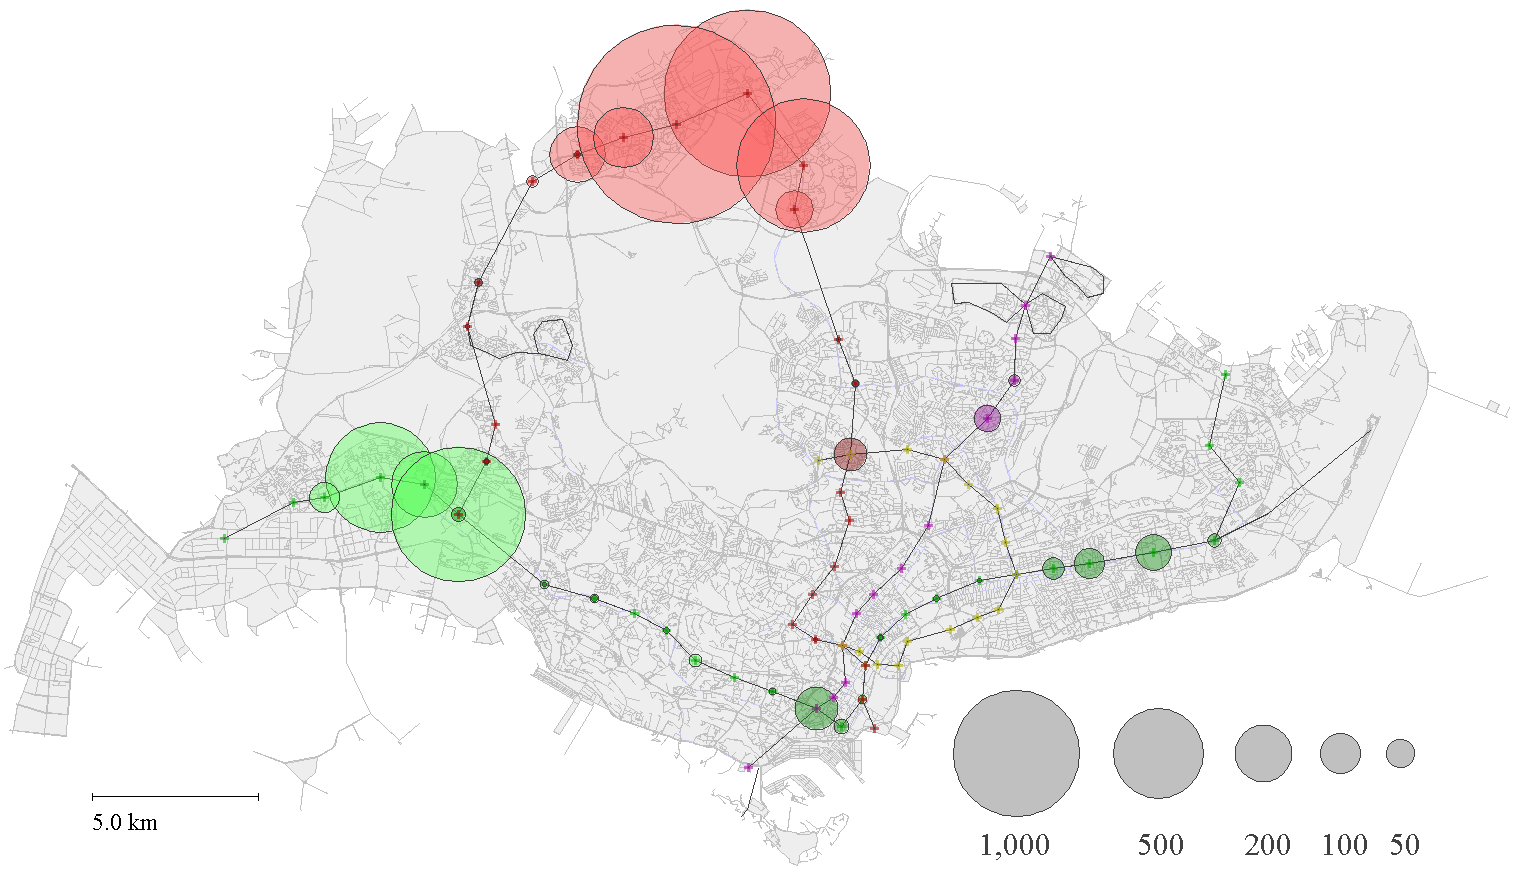
\includegraphics[width=0.25\textwidth, angle=0]{extending/figures/ebr/Backwards.png} \end{center}

\editdone{This text has undergone the professional edit. Please no grammatical changes anymore! They are most-probably wrong.}

\createStandardInformationBasic{{\url{http://matsim.org/javadoc} $\to$ core $\to$ pt package}}{The module is invoked by enabling it in the configuration.}{\lstinline{transit} section(s) of the config file.
}{\citet{Rieser2010,Neumann2014PhD}}
\ah{GTFS2TransitSchedule is also in there!}

% ##################################################################################################################
\section{Modeling Public Transport with MATSim}
\subsection{Introduction}
Public transport---or \emph{transit} as it is sometimes called---plays
an important role in many transport planning measures, even those initially
targeting only non-transit modes. By making other modes more or less
attractive (\eg by providing higher capacity with additional lanes, allowing
higher speeds, or charging money by setting up area road pricing), travelers
might reconsider their mode choice and switch to public transport (\emph{pt})
from other modes, or vice versa. Such changes can also occur when transit
infrastructure is changed; additional bus lines, changed tram routes with
different stops served, or altered headways---all are important for travelers
on specific lines, or public transport in general. Around~2007,
interest grew in extending \gls{matsim} to support detailed simulation of 
modes other than private car traffic, particularly public transport.

In a first step, \gls{matsim} was extended so that modes other than
\emph{car} would be \gls{teleported}; agents would be removed from one location
and placed at a later point of time---corresponding to estimated travel time---at
their destination location, where they could commence their next activity.
Together with a simple mode-choice module, randomly replacing all 
transport modes in all plan legs and a simple travel time estimation for
modes different than \emph{car}, first case studies resulting in modal share
changes were performed using \gls{matsim}
\citep{RieserGretherNagel2008modeChoiceCalculations,
GretherEtAl2009SimpleModeChoiceIPL}. This \gls{teleportation} mode is now available, by
default, in \gls{matsim} and still a very good fallback option to get a \gls{multimodal} scenario
up and running with as little data as possible.

In a second step, \gls{qsim} was extended to support detailed simulation of
public transport vehicles serving stops along fixed routes with a given schedule
\citep{Rieser2010}.
The next section describes, in more detail, data required and resulting features for this
detailed public transport simulation.

% ============================================================================================
\subsection{Data Model and Simulation Features}
\gls{matsim} supports very detailed modeling public transport; transit
vehicles run along the defined transit line routes, picking up
and dropping off passengers at stop locations, while monitoring transit
vehicles' capacities and maximum speeds. Data used to simulate public
transport in \gls{matsim} can be split in three parts:
%
\begin{itemize}\styleItemize
\item Stop locations
\item Schedule, defining lines, routes and departures
\item Vehicles
\end{itemize}

This data is stored in two files; vehicles are defined in one
file, stop locations and schedule in
another.
Examples of such files can be seen in
Section~\ref{sec:inputdata:transitvehicles} and
Section~\ref{sec:inputdata:transitschedule}, respectively.

The data model is comparable to other public transport planning
software, but simplified in several respects. A line typically has two or more
routes; one for each direction and additional routes when vehicles start
(or end) their service at some point on the full route (coming
from, or going to, a depot). Each transit route contains a network route,
specifying on which network links the transit vehicle drives, as well as
a list of departures, providing information about what time a vehicle
starts at the first route stop. A route also includes an ordered list
of stops served, along with timing information specifying when a vehicle
arrives or leaves a stop. This timing information is given as offsets only, to
be added to departure time at the first stop. Each departure contains the
time when a vehicle starts the route and a reference to the vehicle 
running this service. Because timing information is part of the route, routes
with the same stops sequence may exist, differing only in time offsets.
This is often the case with bus lines, that take traffic congestion and
longer rush hour waiting times at stops into account in the schedule. 

Stop locations are described by their coordinates and an optional name; they must
be assigned to exactly one line of the network for the simulation. Thus, they
can be best compared to ``stop points'' in \gls{visum}. There is, currently, no logical
grouping of stop locations to build a ``stop area''; this is a cluster of
stops often sharing the same name, but located on different intersection arms, 
served by different lines, many with transfer corridors for passengers.

Each vehicle belongs to one vehicle 'type', which describes various
characteristics, like seating and standing capacity (number of
passengers), its maximum speed and how many passengers can board or depart
a vehicle per second.

This data model already supports several advanced public transport modeling aspects: 
varying travel speeds along routes during different
times of day (important for improved simulation realism), using diverse vehicle types 
on routes at different times of day (interesting for schedule
economic analysis) and re-using transit vehicles for multiple
headways along one or different routes (allows vehicle deployment planning optimization, 
or research on delay-propagation effects).

With these data sets, the \gls{qsim} will simulate all transit vehicle movements.
The vehicles will start with their first route stop at the given
departure time, allow passengers to enter and then drive along their route,
serving stops. At each stop, passengers can enter or leave the vehicle.
The simulation generates additional, transit-related events whenever a transit
vehicle arrives or departs at a stop, when passengers enter or leave a vehicle,
but also when a passenger cannot board a vehicle because its capacity
limit is already reached. This allows for detailed analyses of \gls{matsim}'s public 
transport simulations.

For passengers to use public transport in \gls{matsim}, they must be able
to calculate a route using transit services. For this, \gls{matsim} includes a public
transport router that calculates the best route to the desired
destination with minimal cost, given a departure time. Costs are typically
defined only as travel time and a small penalty for changing lines, but other,
more complex cost functions could be used.

The routing algorithm is based on Dijkstra's shortest path algorithm
\citep{Dijkstra_NM_1959}, but modified to take
multiple possible transit stops, around the start and end coordinates,
into account to find a route. Multiple start and end stops must be considered
to generate more realistic transit routes; otherwise, agents could
be forced to travel first in the wrong direction, or wait at an infrequently
served bus stop, instead of going a bit further to a busy subway stop location.
By modifying the shortest path algorithm to work with multiple start and end
locations, a considerable performance gain was achieved when compared to the basic (and somewhat naive)
implementation that calculated a route for each combination of start/end location
and then chose the best outcome.
%
%"\Karen{Please check the meaning of this last sentence;
%it was not clear whether the last phrase of the sentence referred to the implementation with
%modifications or the basic version.  Thanks!}"
%\ah{I added ``(and somewhat naive)'' as I think it is quite precise}

% -----------------------------------------------------------------------
\subsection{File formats}

\subsubsection{\lstinline|transitVehicles.xml|}
\label{sec:inputdata:transitvehicles}

%%\kai{convert to normal vehicles?}

%%\ah{copied from let's get started:}
%%\kai{vehicles.xml?  (without ``transit''?)} \kai{Andreas, fyi: I think we are leaning towards having separate containers vehicles.xml and transitVehicles.xml.  Not yet implemented.}

To simulate public transport in \gls{matsim}, two additional input files are necessary. One is \lstinline|transitVehicles.xml|, which describes vehicles serving the lines: big buses, small buses, trains or light rail vehicles and description of each vehicle's passenger transport capacity.

Public transport vehicle description can be split into two parts; first, vehicle types must be described, specifying how many passengers a vehicle can transport (Note that the term ``vehicle'' can refer to multiple vehicles in reality, \eg a train with several wagons should be specified as one long vehicle with many seats). Second, actual vehicles must be listed. Each vehicle has an identifier and is a previously specified vehicle type. The following shows an example of a such a file, describing one vehicle  and two vehicles of the same type. 

\begin{xml}
<?xml version="1.0" encoding="UTF-8"?> 
<vehicleDefinitions xmlns="http://www.matsim.org/files/dtd" 
       xmlns:xsi="http://www.w3.org/2001/XMLSchema-instance" 
       xsi:schemaLocation="http://www.matsim.org/files/dtd http://www.matsim.org/files/dtd/vehicleDefinitions_v1.0.xsd"> 
	<vehicleType id="1"> 
      <description>Small Train</description> 
      <capacity> 
         <seats persons="50"/> 
         <standingRoom persons="30"/> 
      </capacity> 
      <length meter="50.0"/> 
   </vehicleType> 
   <vehicle id="tr_1" type="1"/> 
   <vehicle id="tr_2" type="1"/> 
</vehicleDefinitions>
\end{xml}

% -----------------------------------------------------------------------
\subsubsection{\lstinline|transitSchedule.xml|}
\label{sec:inputdata:transitschedule}
The second, rather complex, file necessary to simulate public transport is \lstinline|transitSchedule.xml|, containing information about stop facilities (bus stops, train stations, or other stop locations) and transit services.

In the first part, stop facilities must be defined; each one is given a coordinate, an identifier and a reference to a network link. The stop can only be served by vehicles driving on that specified link. It is also possible to specify both a name for the stop and whether other vehicles are blocked when a transit vehicle halts at a stop. This last attribute is useful when modeling \eg different bus stops, where one has a bay, while at another, the bus must stop on the road.

After stop facilities, transit lines, their routes and schedules are described. This is a hierarchical data structure; each line can have one or more routes, each with a route profile, network route and list of departures. The following listing is an example of a basic, but complete transit schedule.
%
\begin{xml}
<?xml version="1.0" encoding="UTF-8"?> 
<!DOCTYPE transitSchedule SYSTEM "http://www.matsim.org/files/dtd/transitSchedule_v1.dtd"> 
<transitSchedule> 
   <transitStops> 
      <stopFacility id="1" x="990.0"  y="0.0"   name="Adorf" 
           linkRefId="1" isBlocking="false"/> 
      <stopFacility id="2" x="1100.0" y="980.0" name="Beweiler" 
           linkRefId="2" isBlocking="true"/> 
      <stopFacility id="3" x="0.0"    y="10.0"  name="Cestadt" 
           linkRefId="3" isBlocking="false"/> 
   </transitStops> 
   <transitLine id="Blue Line"> 
      <transitRoute id="1"> 
         <description>Just a comment.</description> 
         <transportMode>bus</transportMode> 
         <routeProfile> 
            <stop refId="1" departureOffset="00:00:00"/> 
            <stop refId="2" arrivalOffset="00:02:30" departureOffset="00:03:00" 
                                                     awaitDeparture="true"/> 
            <stop refId="3" arrivalOffset="00:05:00" awaitDeparture="true"/> 
         </routeProfile> 
         <route> 
            <link refId="1"/> 
            <link refId="2"/> 
            <link refId="3"/> 
         </route> 
         <departures> 
            <departure id="1" departureTime="07:00:00" vehicleRefId="12"/> 
            <departure id="2" departureTime="07:05:00" vehicleRefId="23"/> 
            <departure id="3" departureTime="07:10:00" vehicleRefId="34"/> 
         </departures> 
      </transitRoute> 
   </transitLine> 
</transitSchedule>
\end{xml}

Each transit line must have a unique ID and each transit route has an ID, which must be unique within that one line, allowing the same route ID to be used with different lines. The \lstinline|transportMode| describes network links where the line runs. (Actually, this is not yet in force, although it might be in the future. It would be possible to let a bus run on train links in the simulation.)

The \lstinline|routeProfile| describes the stops this route serves; the route itself describes the series of network links the transit vehicle's driver must navigate, often referred to as network route. Note that the complete route, \ie all links the vehicle traverses, must be listed in the route, not only those with stops. All specified stops should occur along this route in correct order. Time offsets given for each stop in the \lstinline|routeProfile| describe relative time offsets to an actual departure time. If a bus departs at 7\,am, and stop~2 has a \lstinline|departureOffset| 3\,minutes, this must be read that the bus is expected to depart at 7:03\,am from the specific stop. All stops in the route profile must have a departure offset defined, except the last one. All stops, except the first one, can, optionally, have an arrival offset defined. This is useful for large trains that stop for several minutes at a station; helping the routing algorithm find connecting services at the correct time, namely the expected train arrival time.

As the last part of a transit route description, a departures list should be given. Each departure has an ID, which must be unique within the route, giving the departure time at the first stop of the specified route profile. The departure also specifies the vehicle (which must be defined in the previous transit vehicle list) with which the service should be run. 

Because of its complexity, transit schedules often contain small mistakes that will return in an error when the simulation runs. Typical examples include: missing links in the network route, or incorrect defined stop order on the network route. To ensure a schedule avoids such issues before the simulation starts, a special validation routine is available:
%
\begin{lstlisting}
java -Xmx512m -cp /path/to/matsim.jar  
      org.matsim.pt.utils.TransitScheduleValidator  
      /path/to/transitSchedule.xml /path/to/network.xml
\end{lstlisting}
%
If run, this validator will print out a list of errors or warnings, if any are found, or show a message that the schedule appears to be valid.

% ============================================================================================
\subsection{Possible Improvements}
While the ability to simulate public transport was a big advance for \gls{matsim},
several shortcomings still require attention:
%
\begin{itemize}\styleItemize
	\item The data model (and thus, the simulation) does not yet fully support some
	real world transit lines: for example, circular lines with no
	defined start and end cannot yet be easily modeled. Some bus or
	train lines also have stops where only boarding or alighting the vehicle is allowed,
	but not both (\eg overnight trains with sleeper cabins). At the moment, \gls{matsim}
	always allows boarding and alighting at stops, leading to agents \eg using a
	train with sleeper cabins for a short trip; in reality, they would be
	denied boarding without a reservation for a longer trip.
	\item A stop location, as seen by passengers in the real world, is
	typically modeled as a number of stop facilities in \gls{matsim}, detailing 
	different locations where transit vehicles stop (depending on their route and
	direction). For analysis, one is often interested in aggregated values
	for such logical stop locations, not for individual stop facilities.
	Such a logical grouping is still missing in \gls{matsim} data format.
	\item Running simulations with a reduced population sample leads to
	artifacts when public transport is used. In a simulation with a sampled demand,
	network capacity is reduced accordingly, to accommodate the fact that fewer
	private cars are on the road. But because 100\,\% of public transport vehicles
	must run (albeit with reduced passenger capacity), calibration becomes
	difficult. This should be solved, in the future, not by reducing network
	capacity, but by giving each vehicle and agent a weighting, specifying how much each should
	count.
	\item The public transport router available and used by \gls{matsim} by default is
	strictly schedule-based. It assumes vehicles can keep up with the
	schedule and that enough passenger capacity is provided. In some regions, where
	transit is chronically delayed and overcrowded, \gls{matsim}'s router will
	consistently advise agents to use routes that will perform badly in the
	simulation. Additional feedback from the simulation back to the router, as 
	already done in the \gls{matsim} private car router, will be needed.
	\item Last, but not least, the current router, based on a modified shortest path
	algorithm of Dijkstra, can become rather slow and memory-intensive for
	larger areas with extensive transit offerings. Improved algorithms to generate
	the routing graph, or different routing algorithms altogether (like the
	non-graph based Connection Scan Algorithm
	\citep{DibbeltEtAl_BonifaciEtAl_2013}) must be explored in the
	future.
\end{itemize}

% ============================================================================================
\subsection{Applications}
Public transport simulation has been used in myriad applications of
\gls{matsim} world-wide. The following list highlights some of these applications,
pinpointing their special public transport simulation features.

\begin{itemize}\styleItemize
	\item Berlin: the Berlin scenario (see Chapter~\ref{ch:berlinI}) was one of
	the first real applications using public transport simulation in \gls{matsim}.
	The road and rail network, as well as the full transit schedule, was converted
	from a \gls{visum} model. It is still one of the few known models where bus and tram
	lines share a common network with private car traffic, enabling full
	interaction between private and public vehicles (like transit vehicles) getting
	stuck and delayed in traffic jams.
	%
	\item Switzerland: \gls{senozon} maintains a model of Switzerland containing the
	full timetable of all buses, trams, trains, ships, and even cable cars, in the
	Swiss alps. The schedule data is retrieved from the official timetable,
	available in a machine-readable format called ``\gls{hafas} raw data format''.
	%
	\item Singapore: The model of Singapore (see Chapter~\ref{ch:singapore}) makes
	heavy use of public transport, and continually pushes the boundaries of what is
	currently possible to simulate. Due to the very large number of buses on
	Singapore's roads and strong demand for public transport, many extensions had to
	be implemented to realistically model pt in this context.
	%
	\item Minibus: The minibus contribution (see next Section~\ref{sec:paratransit}) 
	added an optimization layer to public
	transport functionality in \gls{matsim}, allowing automatic
	generation of an optimized transit schedule for a specific region.
	%
	\item WagonSim: In the WagonSim contribution (see Chapter~\ref{ch:wagonSim})
	public transport simulation was used to simulate
	rail-bound freight traffic. While the simulation was still moving around
	transit vehicles and letting passengers enter and leave these vehicles, the scenario
	had been customized so that vehicles corresponded to freight trains and
	passengers corresponded to actual goods being transported. Custom
	implementations of transit driver logic replaced vehicle capacity definition 
	by an alternative definition, ensuring that the trains vehicles represent
	did not get too long or heavy. The network was constructed so that changing
	vehicles at stops took minimum time, corresponding to the time
	needed for switching wagons at freight terminals.
\end{itemize}

In addition to applications mentioned in the list above, many additional scenarios now
use public transport simulation in \gls{matsim}. Importantly, the list also
shows, that with some custom extensions and imagination, public transport
functionality can be used for far more than ``just simulating public transport''; it can be
employed to solve complex problems previously handled by operations research
groups.

% ##################################################################################################################
\section{Paratransit}
\label{sec:paratransit}
Paratransit is an informal, market-oriented, self-organizing public transport system. 
Despite the significance of this transport mode, it is mainly unsubsidized, relying on collected fares. 
Paratransit systems can be categorized by route pattern and function, by driver organization, type of stops and fare type. 
Most case studies covered by the \citet[][]{Neumann2014PhD} thesis indicate that paratransit services are mainly 
organized as route associations operating 8-15\,seater vans on fixed routes. Most of the services run in direct competition to a
public transport system belonging to a public transit authority. Such a service---minibuses with fixed routes, but without fixed schedule---is often called a jitney service.
The minibus module of \gls{matsim} is based on the most common characteristics, with the understanding that the jitney/minibus
service is only one of many possible paratransit services.

The minibus model is integrated in the \gls{multimodal} multi-agent simulation of \gls{matsim}. In the model, competing minibus operators begin to explore the public transport market, offering their services. With more successful operators expanding and less successful operators going bankrupt, a sustainable network of minibus services evolves. In \citet[][]{Neumann2014PhD}, the model is verified through multiple illustrative scenarios, analyzing the model's sensitivity to different demand patterns, transfers, and interactions of minibuses and a formal operator's fixed train line.

The minibus model can be applied to two different transport planning fields. First: in the simulation of real paratransit targeting the inner workings of different paratransit stakeholders' relationships, the model can create ``close-to-reality'' minibus networks in a South African context. \citet[][]{NeumannEtAl2014MinibusRSA} gives an in-depth presentation of the module application and South African paratransit in general. Given the informal and emergent nature of minibus paratransit in developing countries, routes, schedules and fares are usually not published; they can only be captured in the tacit knowledge of operators and frequent users. Applying the minibus model has proven valuable in gaining a better understanding of how routes evolve. Instead of imposing routes and schedules \emph{on} the \gls{matsim} model, as is usually the case for formal transit, the modeler observes and gets the paratransit routes as an output \emph{from} the model. As each operator aims to maximize their profit, the resulting network often favors the operators' business objectives, instead of the connectivity and mobility of the mode's users. This model feature accurately captures route-forming behavior in the South African case, where commuters are often required to take multiple, longer trips instead of direct trips.

Second, the same model provides a demand-driven approach to solving a formal transit authority's network design problem; it can be used as a planning tool for the optimization of single transit lines or networks. For more details on the second form of application,see Section~\ref{sec:paratransit_application}.

For further reading: \citet[][]{Neumann2014PhD} provides an understanding of the underlying principles of paratransit services, namely minibus services, its stakeholders, fares, route functions, and patterns. Furthermore, it contains an in-depth description of the minibus model, its theoretical background, and its application to illustrative scenarios, as well as real world examples. The website of \gls{matsim} also hosts latest implementation documentation at \url{http://matsim.org/doxygen}.

% ##################################################################################################################
\section{Network Planning or Solving the Transit Network Design Problem with MATSim}
\label{sec:paratransit_application}
%\ah{Hilft da wagonSim oder dass was die IVT.Weidmann-Gruppe gerade macht?}
%\an{Braucht's eigentlich nicht aber man kann die beiden Koppeln und entsprechend auch Gueterfluesse optimieren.}
%
A public transport system's success depends primarily on its network design. When transport companies try to optimize a line using running costs as the main criteria, they quickly find that demand must be taken into consideration. The best cost structure is unsustainable if potential customers leave the system and opt for alternatives, like private cars. The basic problem to solve: find sustainable transit lines offering the best possible service for the customer.

More specifically,
\begin{itemize}\styleItemize
\item The customer's demand side asks for direct, uncomplicated connections.
\item The operator's supply side asks for profitable lines to operate.
\end{itemize}
Informal public transit systems around the world, often referred to as paratransit, are examples of market-oriented, self-organizing public transport systems. For an in-depth coverage of paratransit, see Section~\ref{sec:paratransit}, with references. Despite the significant and increasing importance of this transport mode, it is mainly unsubsidized and relies only only on collected fares. Thus, the knowledge of paratransit---and its ability to identify and fill market niches with self-supporting transit services---provides an interesting approach to solving a formal public transit company's network design problem.

\noindent
The minibus module of \gls{matsim} provides a demand-driven approach to solving a formal transit authority's network design problem; it can be used as a planning tool for the optimization of single transit lines or networks. In the \citet[][]{Neumann2014PhD} thesis, the model was applied to two different Berlin public transit authority, \gls{bvg}'s, planning problems. In the first scenario, the model constructed a transit system, from scratch, for the district of Steglitz-Zehlendorf. The second scenario analyzed the Tegel airport closure impact on \gls{bvg}'s bus network. Apart from Tegel itself, the rest of the bus network was unaffected by the airport closure. The resulting minibus model transit system resembled the changes \gls{bvg} had scheduled for Tegel's closure.

In conclusion, the minibus model developed in the thesis automatically adapted supply to demand. The model not only grew networks from scratch, but also tested an existing transit line's sustainability and  further optimized the line's frequency, time of operation, length, and route. Again, the optimization process was fully integrated into the behavior-rich, multi-agent simulation of \gls{matsim} environment, reflecting passenger reactions, as well as those from competing transit services and other road users. Thus, the minibus model can be used, along with more complex scenarios, like city-wide tolls or pollution analyses.

% ##################################################################################################################
\section{Public Transport in Singapore}
% ============================================================================================
\subsection{Semi-Automatic Tool for Bus Route Map Matching}
\label{sec:SemiTool}
Current public transport assignment models adapt network assignment models to work with public transport traffic. Many commercial software products like \gls{emme2}, \gls{visum} and \gls{omnitrans} offer sophisticated procedures that include timetable-based route search. However, these models do not include interaction between public transport services and private transport. As mentioned above, the \gls{matsim} implementation handles private car traffic and public transport traffic in an integrated way, but it needs accurate public transport line routing on the transport network. While this is usually straightforward for rail-based public transport modes, the routing problem for buses requires more attention; experience shows that assumption of a shortest-path between two consecutive stops leads to unsatisfactory results. To overcome this shortcoming, one can either draw the routes manually or employ map-matching algorithms dependent on tracking data. Due to the burden of manual procedures, and the increasing availability of \gls{gps} tracking data, map-matching is becoming increasingly relevant. However, common map matching algorithms are usually not designed to account for the peculiarities of public transport routing; the procedure is very sensitive to errors in network coding, inaccurate bus stop locations and the simplified  link shapes in the model.

This section presents a semi-automatic procedure combining public bus routes information (sequences of consecutive stop locations and sequences of geo-referenced points) with a high resolution network \citep[][]{Ordonez_HKSTS_2011}. The objective is to obtain a sequence of links for every route of every line and to associate each bus stop with one single link in the network. The procedure was designed to prepare the Singapore scenario public transport extension, but the tools developed can be used to set up any other scenario with similar initial data (timetable and high resolution network).

% -----------------------------------------------------------------------------------
\subsubsection{Problem Definition}
Generally, the problem can be defined as follows. Given:
%
\begin{itemize}\styleItemize
\item A set of stop locations (two-dimensional point coordinates);
\item A set of route profiles (sequence of consecutive stops);
\item A set of \gls{gps} points sequences (sequence of two-dimensional point coordinates);
\item A high resolution navigation network (two-dimensional directed graph with attributes);
\end{itemize}
%
the task is to associate each stop with a network link, and translate each route to a network path (connected sequence of links). Figure~\ref{fig:Problem} illustrates the problem by providing an example of the available input information and correct output.
%
\createfigure
{Input data and expected solution of the map-matching problem}
{Input data and expected solution of the map-matching problem}
{\label{fig:Problem}}
{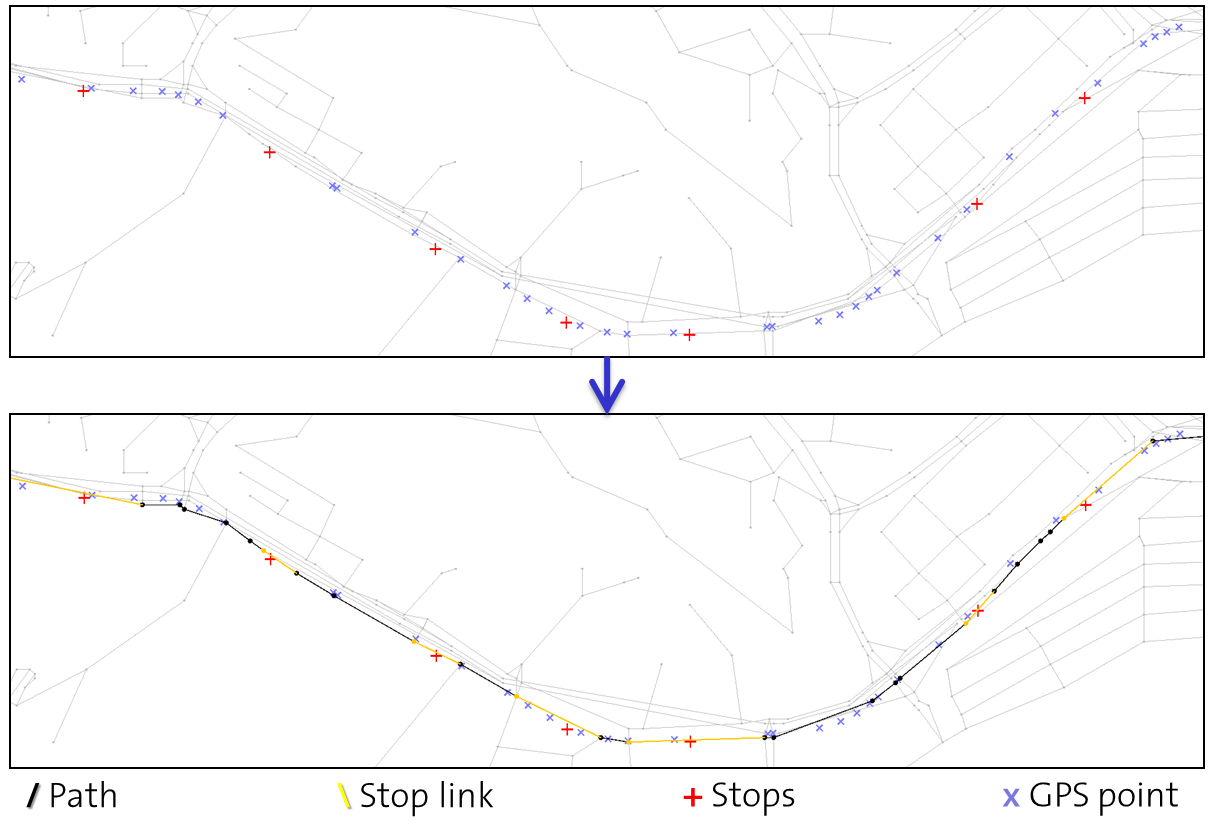
\includegraphics[width=1.0\textwidth]{extending/figures/semiAuto/Problem.png}}
{}

% .....................................................
\paragraph{Input Information}

The \gls{gtfs} is a recent, but already widely-used format for specifying public transport systems, created by Google for feeding its geographic information applications. As of April~2011, the Singapore public transport system featured 4\,584\,bus stops serviced by 355\,bus lines, all recorded on \gls{gtfs}. Each line had several routes, i.e. different outward and return routes (due to one-way streets), as well as different coverage of serviced bus stops on weekdays and weekends. \gls{gtfs} records the name and location of each bus stop; for bus lines, it records constituent bus routes as a sequence of stops, along with their shape (a sequence of \gls{gps} points) as additional information. 

The \gls{gtfs} data must be mapped to a high resolution network; for Singapore, this is a navigation network developed by \gls{navteq}. The network is a directed graph where streets and intersections are represented as links and nodes. The links between nodes record attributes like street name, number of lanes, length, flow, free speed and capacity. Nodes are simply recorded as two-dimensional point coordinates. This network has a total of 79\,835\,links and 43\,118\,nodes.

% .....................................................
\paragraph{Special Restrictions}

There are some intrinsic characteristics of the public transport system that should be considered serious restrictions. First, when a certain stop is assigned to a network link, this link should be a part of all paths belonging to this stop's routes. In other words: once established, stop-link relationships are fixed for resolving the missing routes. If the \gls{gps} points from a route including a specific stop suggest it should be associated with a different nearby link, then all other routes including that stop must be resolved again. Hence, the order in which the routes are resolved is important; it is preferable to resolve those routes first, when we completely trust supporting information quality (\eg \gls{gps} trails).

Second, while many lines run in two directions, with most bus stops having a corresponding stop in the opposite direction (stop located on the other side of the street), this cannot be used to our advantage, because links defined by each return route are different, locations of stops are not necessarily exactly opposite to those in the opposite direction and return routes  don't always use the same street.

However, some routes on the same line have an inclusion relationship; in peak hours, segments of bus routes with high demand are served by additional buses running on partial routes to meet demand. In these cases, if a full route is resolved, its partial routes solutions are included.

% ---------------------------------------------------------------------------
\subsubsection{Solution Approach}
It is not possible to automatically map-match the given \gls{gps} po with the network, as standard methods usually require at least 10\,points for each link \citep[][]{SchuesslerAxhausen_TechRep_IVT_2009}. In the Singapore \gls{gtfs}, distance between consecutive points averages about 65\,meters, and average link length is about 91\,meters; thus, we have fewer than 2\,points per link, on average. Furthermore, not all the routes have \gls{gps} points, which inhibits using a full automatic solution; in the Singapore \gls{gtfs}, there are 38\,bus routes without \gls{gps} points.

Consequently, the strategy for resolving each route consists of a semi-automatic procedure. Figure~\ref{fig:Process} illustrates the process. First, a simple map-matching algorithm is applied if the route is not part of a bigger route already solved (inclusion relationship described above). In this case, only a previous solution's partition is needed to obtain a first solution. Then, an automatic verification (described below) is performed. If the verification ends with a positive outcome, one can decide to finish the route and save the solution, or to continue editing. If one decides, or is forced, to modify the solution, there are two ways to proceed: changing parameters and running the automatic algorithm again, or editing the solution interactively with a graphical interface editing tool. In both cases, automatic verification must be executed again. If previously saved stop-link relationships are modified, prior routing solutions containing one of the involved stops are erased.
%
\createfigure
{Semi-automatic process for one route}
{Semi-automatic process for one route}
{\label{fig:Process}}
{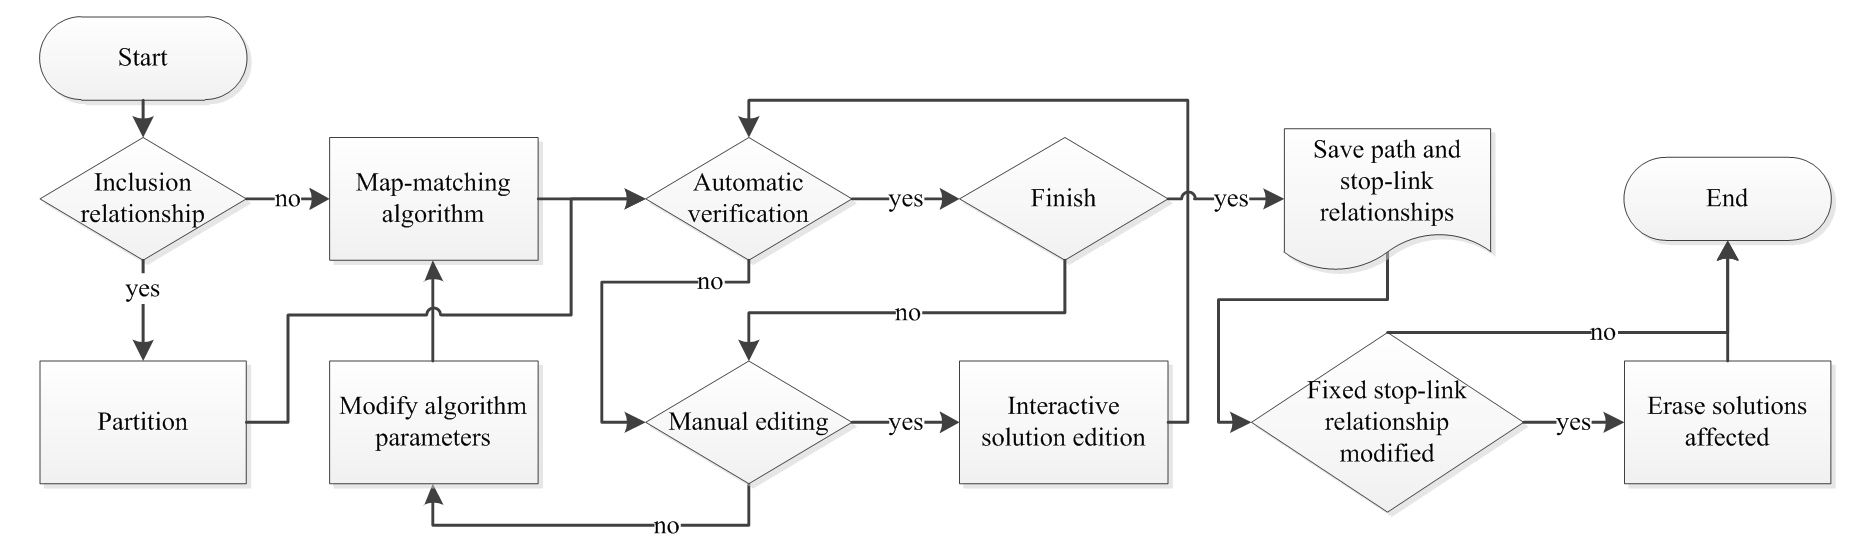
\includegraphics[width=1.0\textwidth]{extending/figures/semiAuto/Process.png}}
{}

As long as more solutions are obtained, it becomes easier and faster to solve further routes, similar to a  machine learning process. This happens for two reasons; first, because of the inclusion relationships that omit the algorithm and second because the increasing number of fixed stop-link relationships relaxes the algorithm  (functioning explained in the following section).

% ---------------------------------------------------------------------------
\subsubsection{Map-Matching Automatic Algorithm}
This algorithm's objective is to generate a solution (path or sequence of connected network links and a set of stop-link relationships) for one route, knowledge of its profile, a sequence of \gls{gps} points and a set of stop-link relationships. The algorithm is designed to deal with:
%
\begin{itemize}\styleItemize
\item	Low \gls{gps} point resolution;
\item	Sporadic low network spatial resolution;
\item	Long distances between two express routes stops;
\item	Understanding that the nearest link to a stop point is not always the correct one.
\end{itemize}

The route map-matching process is illustrated in Figure~\ref{fig:Algorithm}. Except for the first stop, the algorithm solves for each stop in the route profile, a portion of the links sequence (from previous to current) and, if this stop has no fixed link, a set of link candidates pooled from the one link selected.
%
\createfigure
{Map-matching algorithm}
{Map-matching algorithm}
{\label{fig:Algorithm}}
{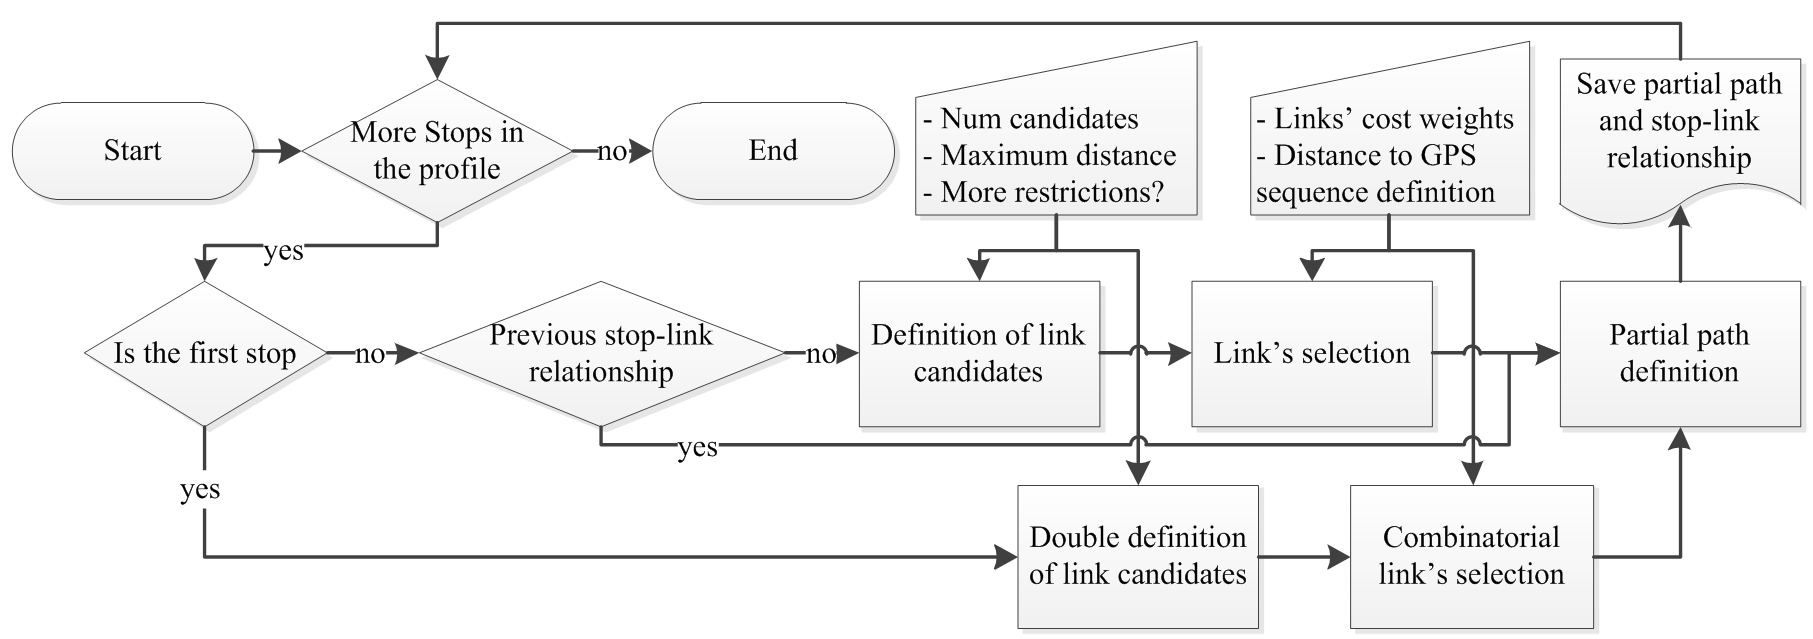
\includegraphics[width=1.0\textwidth]{extending/figures/semiAuto/Algorithm.png}}
{}

Link candidates are defined as follows: the $NL$ closest links to the stop point, within a distance $D_{max}$, define a set of candidates. Each set's element could be subjected to more restrictions; the closest point, between the stop point and the infinite line defined by the link, must be inside its line segment and the angle between the link direction and the nearest \gls{gps} points sequence direction must be lower than $\alpha_{max}$.

The link's selection is performed as follows; from the previous stop link to each defined candidate, an A star search algorithm is applied for finding the shortest path. For running this algorithm, each link's cost depends on the link's travel time and distance to the \gls{gps} points. A product with flexible exponents was proposed as a first model:
%
\begin{equation}
\label{eq:LinkCost}
	C_{link} = \exp{\frac{L_{link}}{S_{link}}}{w_{1}}\exp{D_{GPS}}{w_{2}}
\end{equation}
%
where $L_{link}$ is its length, $S_{link}$ is its free speed, $D_{GPS}$ is its distance to the \gls{gps} points sequence and $w_{1}$ and $w_{2}$ are positive weights with a standard value of 1, but modifiable by the user, according to existence or quality of the \gls{gps} points sequence. The definition of $D_{GPS}$ can also be modified; in the simplest approach, it is the minimum distance between the link and all \gls{gps} points (point-segment distance). From all calculated paths, the shortest is selected and added to the general route solution. The corresponding link candidate is also related to the stop. 

If the current stop has a stop-link relationship, only the shortest path to this stop defines the solution. Thus, the process continues with the next stop in the route profile. If the first stop of the profile has no fixed link, a similar algorithm between the first and the second stop is performed. The definition of candidates' procedure is applied to the first and the second stops. Then, the candidates' selection procedure consists of obtaining the shortest path of all combinations between the two sets of candidates, then selecting the shortest one. This path defines links for both stops.

% ---------------------------------------------------------------------------
\subsubsection{Automatic Verification}
In this step, accuracy of the routing solution is automatically checked by performing the following ordered verification:
%
\begin{enumerate}\styleEnumerate
\item Is the path joined?
\item Is the path without U turns?
\item Is the path without repeated links?
\item Does every stop of the route have a stop-link relationship?
\item Is every link related to a stop inside the path?
\item Is the related links' order in the path the same as the corresponding stops' order in the route profile?
\item Is the nearest point between the stop point and the infinite line defined by the link inside its line segment in every stop-link relationship?
\item Are the first and last links of the path related to the first and last  stops of the route profile?
\end{enumerate}

Verifications (2), (3) and (7) are not mandatory and can be deactivated through the user interface. User interaction is necessary to (i) cover possible errors, and (ii) include actual route characteristics: some bus routes do include U turns, some repeat exactly the same street, in the same direction, during their travel and the geometric restriction presented in (7) is not always valid in big stop facilities, like bus interchanges.

% ---------------------------------------------------------------------------
\subsubsection{Manual Editing Functionalities and Implemented Software}
The edit functions' objective is to allow the user to modify the automatically generated routing solution. Even if the automatic algorithm generates a correct solution based on input data, problems like recent changes in routes, differences in release dates between \gls{gps} points and network data, erroneous \gls{gps} points, or lack of network element all require manual changes. Although one also could modify and correct the input data, or the generated solution, with direct data modifications, two-dimensional visualization and keyboard-mouse user interaction are two quality attributes that help reduce time and effort. Developed functional requirements and quality attributes are:
%
\begin{enumerate}\styleEnumerate
\item Visualization: A navigation network is displayed, including all relevant information for working with a single route. This includes the route's profile, given sequence of \gls{gps} points, and its current solution (path and stop-link relationships). Selected elements are drawn in a different color. Everything is displayed in a two-dimensional and interactive way, including the cursor location in working coordinates, panning, zoom and view-all options.
%
\item Selection: Different options for selecting solution elements, or elements from the network, are provided. It is possible to select the nearest link from the solution or from the network, the nearest node from the network, or the nearest stop from the solution, to a point indicated by the user. When a stop that already has a stop-link relationship is displayed, its corresponding link is highlighted as well. If a solution path link is selected and does not have a subsequent link connected, a new one from the network is selected with one click; the selected link is that with the angle most similar to the line defined by the end node of the initial link and a point indicated by the user.
%
\item Path modification: The first link of the sequence can be added by selecting any network link. If a solution path link does not have a subsequent link connected, it is possible to add one, according to the selection function described in (2). If there are two unconnected sequential links in the solution (a gap), a sub-sequence  connecting these links is added, using the shortest path algorithm, with the current parameters. Further, selecting one  solution path link, it is possible to delete it, or to delete all links before or after it. Finally, stop-link relationships can be modified by selecting either elements. If the modified relationship was fixed, the user is prevented from modifying the relationship, because the tool will erase the solutions of the routes to which the selected stop belongs.
%
\item Network modification: New nodes to the road network can be added. In addition, with any node selected, it is possible to add a new link selecting the end node.
\end{enumerate}

These functions were implemented in a software package developed from scratch in \gls{java} and using the Java2D library for graphics. The package reproduces the described solution approach, looking for non-solved routes, and running the map-matching algorithm and the automatic verification for each one. Figure~\ref{fig:Application} shows the user interface and a demo video can be accessed at \url{http://www.vimeo.com/27137889}.

\createfigure
{User interface of the application to edit automatic solutions}
{User interface of the application to edit automatic solutions}
{\label{fig:Application}}
{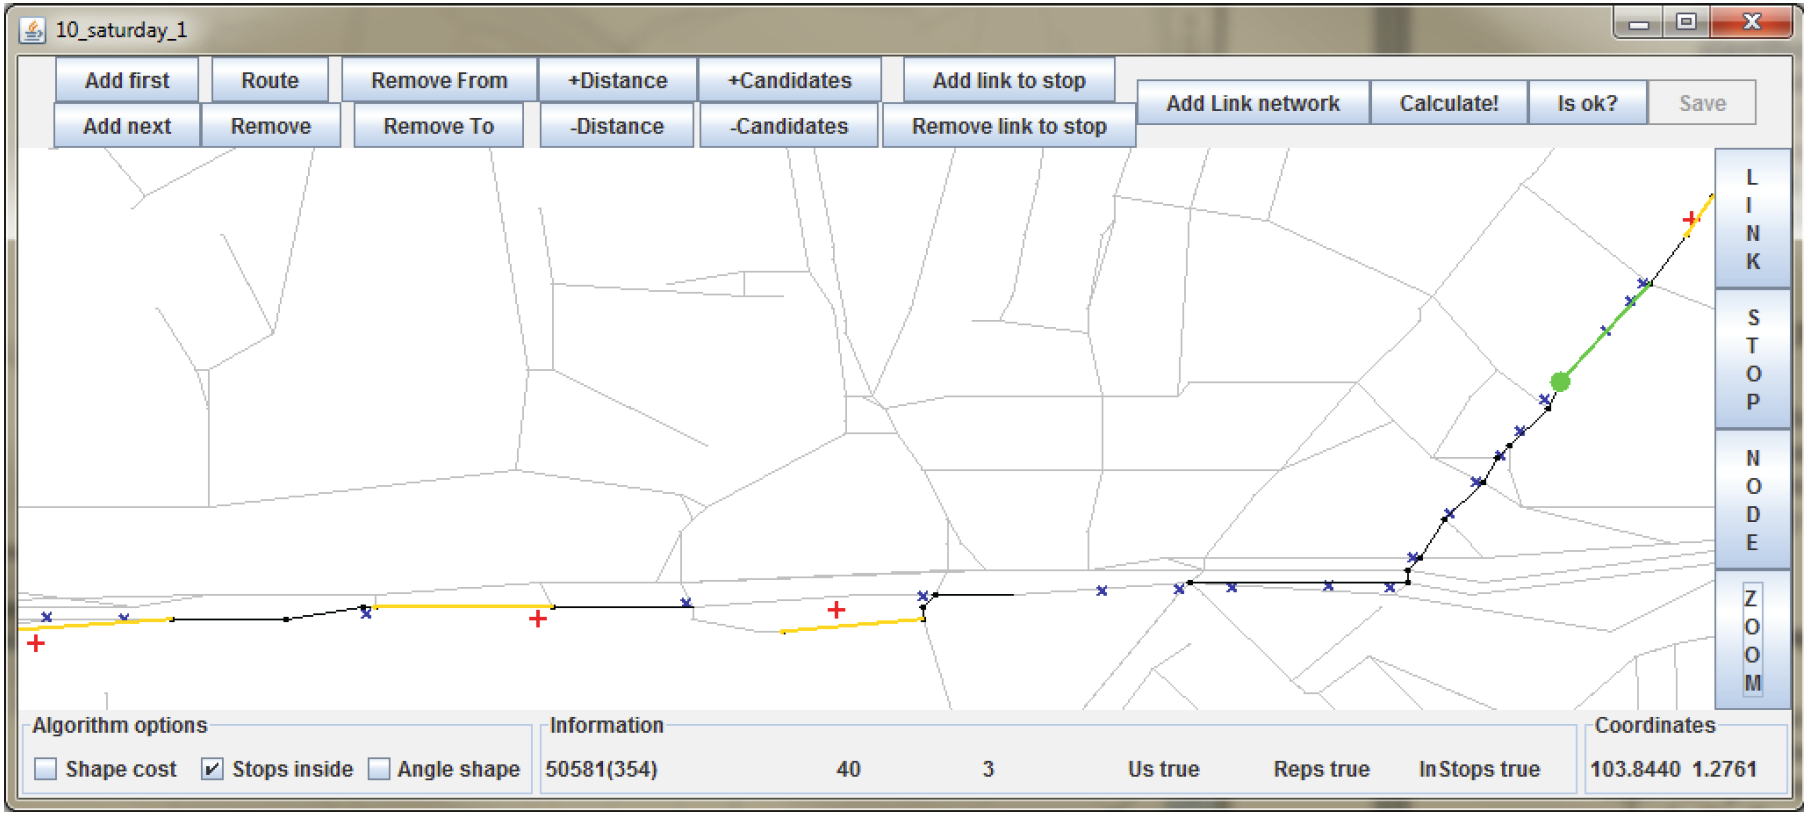
\includegraphics[width=1.0\textwidth]{extending/figures/semiAuto/Application.png}}
{}

% ---------------------------------------------------------------------------
\subsubsection{Conclusion and Outlook}
The semi-automatic procedure designed for map-matching bus lines with a high resolution navigation in Singapore was successful, allowing the solving of all bus routes and stops in only ten days, even taking into account the quality of the input information offered, highlighting the low spatial and temporal resolution of the \gls{gps} points given for each route. Analysis indicates that reducing manual modification time is the best way to improve the procedure, which can be done by modifying the automatic algorithm to obtain more accurate results for the initial routes to be solved, or in other words, for routes not affected by the learning process.

As \gls{gtfs} is becoming so popular for defining public transport systems and the code in which this process is implemented is open source, it can be used for matching routes with high resolution networks of any \gls{gtfs}-specified place. The tools are available as a \gls{matsim} \gls{contribution} (\lstinline|GTFS2TransitSchedule|). For generating \gls{matsim} simulation scenarios, the procedures have been used by research teams in the province of Gauteng, South Africa, on the Toronto scenario and on a different public transport simulation model developed by SMART-MIT in Singapore.

% ============================================================================================
\subsection{New Dynamic Events-Based Public Transport Router}
In public transport route choice, decisions and actions of a particular user depend not only on his/her own preferences, like value of time, crowd avoidance or willingness to pay. They also depend on the decisions and actions of many other public transport users, operators and authorities. Even private transport users' decisions are also involved, as everybody shares the same infrastructure.

This implementation of \gls{matsim} used a \gls{sbptr}, as mentioned above, meaning that when an agent needed a route for a given start time, origin and destination, the \gls{sbptr} found the shortest path in a schedule-based network (assuming public transport vehicles are always on time and always have space). Within the mobility simulation, a vehicle could arrive early or late and/or it could be full, thus not allowing additional passengers to board. With a negative result, the agent obtained a bad score and this plan would have probably been replaced with a more favorable one during the iterative learning process. This scenario's problem occurred when the agent tried to find a new route for the same start time, origin and destination, the public transport scheduled network shortest path remained the same; agents could not improve their experiences by changing the route.

To address this shortcoming, a new \gls{ebptr} was proposed \citep[][]{OrdonezErath_TechRep_FCL_2013}, modeled, implemented and tested. It took the given schedule as a base for the first iteration, but updated information on travel times, occupancy of the public transport vehicles, and waiting times was propagated between subsequent iterations. Thus, when same day executions were performed, new routes could be generated for the same start time, origin and destination, because the system is remembered delayed bus services (longer travel times), or train services where the vehicle arrived full (longer waiting times). However, the network used to route agents required a new topology to account for such variables. This approach allowed then to account for emergent phenomena; in situations where overcrowded vehicles prohibited boarding, it made sense for some agents to travel a few stops in the outbound direction. They could then transfer to an inbound vehicle with sufficient capacity and board. Although more memory was needed, similar or even better computation times were achieved when shortest path calculations awe performed, due to the simpler network topology. Furthermore, to achieve user equilibrium required a significantly smaller number of iterations.

% ---------------------------------------------------------------------------
\subsubsection{Events-Based Public Transport Router} 
\label{sec:RouterStructure}
A new \gls{ebptr} was developed for \gls{matsim} to more realistically model public transport route choice, where agents learn, over time, that transit vehicles are not always on time, do not always have sufficient space to allow boarding and trips with more comfort are often preferable.

% .....................................................
\paragraph{Network Topology}

Figure~\ref{fig:Networks}(b) shows the structure of the proposed public transport network, compared with the original structure (Figure~\ref{fig:Networks}(a)). Inspired by the network designed by \citet{SpiessFlorian_TransResB_1989} this implementation had two types of nodes. The first type represented a stop facility (green-black squares) as point in space, while the second type (yellow-red dots)represented a stop-route relation which could be seen as a physical or virtual platform for each line  passing a particular stop facility. For example, different platforms in a metro system needed to be modeled as different stop facilities, because different services arrived at each platform and walking paths were needed to change from one platform to another. For bus stop facilities, they represented virtual platforms; in reality, buses from different lines serving the same bus stop would normally use the same physical infrastructure \eg a bus bay. To connect those nodes, there were four types of links. The in-vehicle links joined two consecutive stop-route nodes in the direction of the correspondent route. The boarding links connected a stop node with each corresponding stop-route node. The alighting links were opposite, connecting stop-route nodes with their corresponding stop node. Finally, walking links connected a stop node with all other stop nodes located within walking distance.

\createfigure
{Comparison of the network topologies}
{Comparison of the network topologies of the schedule-based transit router (a) and the new events-based transit router (b)}
{\label{fig:Networks}}
{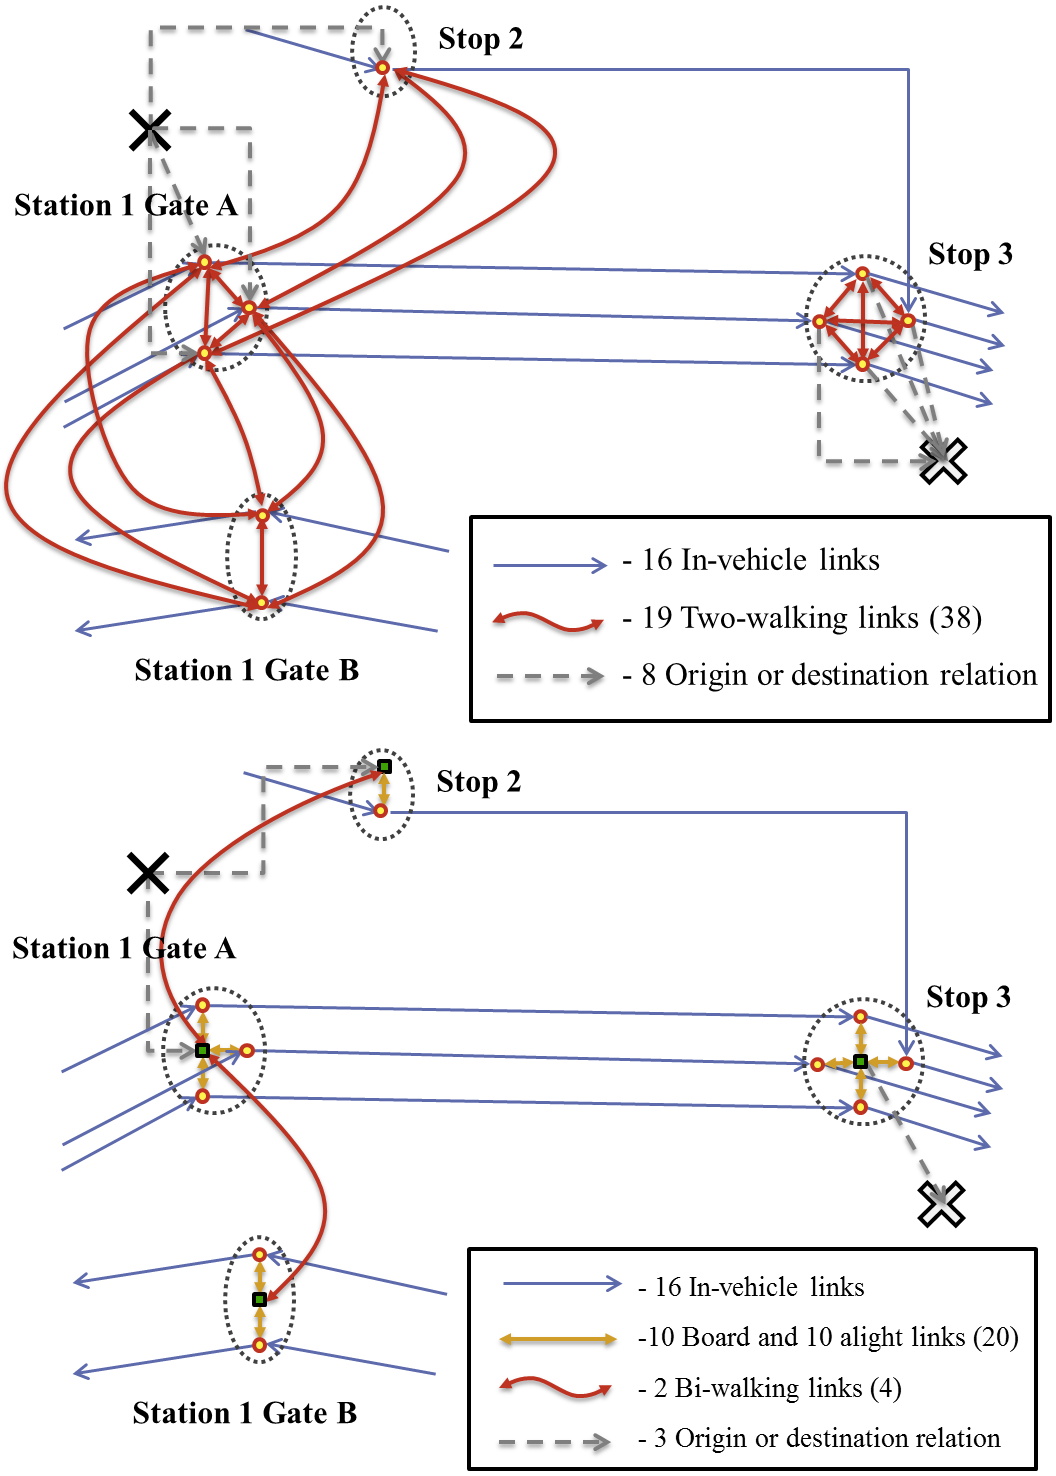
\includegraphics[width=1.0\textwidth]{extending/figures/ebr/Networks.png}}
{}

% .....................................................
\paragraph{Link Costs}

Each link in this network had a related time-dependent disutility function. Different costs were saved for different times in the day for a given time bin (at this time, 15\,minutes). In-vehicle link disutilities depend on vehicle travel time, travel distance, level of occupancy and a fare rate, if this system is distance-based. Boarding link disutilities depended on waiting times, a transfer cost, and a fixed fare if this system was entry-based; thus it was possible to relate specific stop-route waiting times to these links. As the first waiting link was not a transfer, this cost had to be subtracted from the whole path cost, but this detail did not affect the shortest path calculation. Alighting links had no associated cost, but a fare could be related to them. Finally, walking links depended on the walking travel time and distance. Equation~(\ref{eq:CostFunction}) shows linear versions of these functions used in this model assuming a distance-based fare system.
%
\begin{equation}\label{eq:CostFunction}
	\begin{array}{l}
		C_{iv}(t) = (\beta_{iv}*t_{iv}(t))(1+g(p_{oc}(t))) + \beta_{vd}*l_{iv} + f_{iv}*l_{iv}\\
		C_{bo}(t) = \beta_{wt}*t_{wt}(t)) + c_{tr}\\
		C_{al}(t) = 0\\
		C_{wk}(t) = \beta_{wk}*t_{wk} + \beta_{wd}*l_{wk}\\
		C_{path}(t) = \sum{C_{iv}(t')} + \sum{C_{bo}(t')} + \sum{C_{al}(t')} + \sum{C_{tr}(t')} - c_{tr}
	\end{array}
\end{equation}

$C_{path}$: Total cost of the path.

$C_{iv}$: Cost of one in-vehicle link.

$C_{bo}$: Cost of one boarding link.

$C_{al}$: Cost of one alighting link.

$C_{wk}$: Cost of one walking link.

$\beta_{iv}$: Personalized cost per unit of time traveling in a vehicle.

$\beta_{vd}$: Personalized cost per unit of distance traveling in a vehicle.

$\beta_{wt}$: Personalized cost per unit of time waiting in a stop.

$\beta_{wk}$: Personalized cost per unit of time walking.

$\beta_{wd}$: Personalized cost per unit of distance walking.

$c_{tr}$: Personalized cost for make a transfer

$f_{iv}$: Vehicle dependent fare rate by distance traveled

$t_{iv}(t)$: In-vehicle travel time (from Stop-stop travel times structure).

$t_{wt}(t)$: Waiting time (from Stop-route waiting times structure).

$t_{wk}$: Walking time.

$l_{iv}$: In-vehicle distance.

$l_{wk}$: Walking distance.

$p_{oc}(t)$: Occupancy level in the in-vehicle link (from Route-stop occupancy structure).

$g(p)$: Simplified function of how occupancy level increases the cost (Equation~(\ref{eq:Occupancy}))

\begin{equation}\label{eq:Occupancy}
	g(p)=\left\{\begin{array}{l}
	0\hspace{25 mm}if\hspace{5 mm}p \leq p_{sit} \\
	r_{sta}*p + b_{sta}\hspace{5 mm} if\hspace{5 mm}p_{sit}<p<1\\
	b_{full}\hspace{20 mm} if\hspace{5 mm}p=1
	\end{array}\right.
\end{equation}

$p_{sit}$: Occupancy level when no more seats are available.

$r_{sta}, b_{sta}$: Parameters of percentage increase in discomfort from standing in the vehicle.

$b_{full}$: Maximum percentage increase when the vehicle is full.

% .....................................................
\paragraph{Shortest Path Algorithm}

To find a public transport route between an origin and a destination, for a given time of day, the applied method was the same as currently implemented in \gls{matsim}; first, the algorithm looked for the stop-nodes within walking distance from both origin and destination. An initial cost was associated with each of these stop-nodes, according to access and egress walking times. Then, starting from all the origin-stop-nodes with a given access cost, a multi-node time dependent Dijkstra algorithm found the shortest path, to the destination-stop-nodes with related egress costs. Thus, the path determined the best \gls{od} combination as well. The algorithm was time-dependent because it recognized that while it proceeded through the path, time advanced; thus, different costs are obtained from the links while time advanced. The total disutility of this path was compared with the cost of a full walking trip. If the cost is less, the path is converted to a sequence of stages: in-vehicle stages for each in-vehicle link in the path and walking stages for each walking link. Boarding and alighting links were ignored for this conversion.

% .....................................................
\paragraph{Structures to Save Travel Times, Waiting Times and Vehicle Occupancy} 
\label{subsec:Structures}

As mentioned earlier, the \gls{mobsim} of \gls{matsim} generated atomic units of information called \glspl{event}, which described changes for each person, \eg boarding or alighting: each vehicle, \eg entering and leaving a link during the simulation. The goal was to save information on public transport experience in one simulation and find better public transport routes for agents in the next iteration. This feedback mechanism was already implemented in \gls{matsim} for private transport; the car router used each saved link's time-dependent travel times from a previous iteration to calculate better routes in the road network, by changing the costs of the links. To allow the \gls{ebptr} to learn from the previous iteration, information about a) stop-stop travel times, b) stop-route waiting times and c) route-stop-stop vehicle occupancy, was required.

\begin{itemize}\styleItemize
\item Stop-stop travel times: to account for public transport vehicle delays, travel time between consecutive stops had be saved. Two stops are consecutive if they were consecutive for at least one public transport route. A first option was using the previously discussed travel times structure that saved time-dependent travel times for each road network link. Because a vehicle had to follow known road links between two consecutive stops, these travel times could be summed. One problem: this structure accounted for all the vehicles in the network, but  travel times of cars and buses were very different, particularly in links with public transport stops. Thus, a special structure was implemented to save these stop-stop travel times. The structure averaged all the public transport vehicle times from one stop to the next during a certain time bin. More specifically, each value comprised the time from when the vehicle arrived at a certain stop until it arrived at the next stop, denoted in the simulation by consecutive \lstinline|VehicleArrivesAtFacility| events. This meant that the first stop waiting time and all queue times (if the vehicle had to queue before the bay or platform was available) were included. In other words, when an agent routed the first in-vehicle link of each trip, the full dwell time would be included. Hence, this agent assumed it was the first passenger entering the vehicle. For all the other in-vehicle links the in-vehicle waiting was included. These stop-stop times were the main component of the in-vehicle link disutilities.
%
\item Stop-route waiting times: Waiting times are a fundamental aspect of public transport route choice and can be long due to vehicle delays (\ie due to the stop location), or full public transport vehicles of one or several consecutive services(\ie due to the route demand and stop position within the route). For that reason, waiting times were saved for each stop-route relation. Similarly, the structure averaged all agent waiting times in a certain stop, for a certain route, during a certain time bin in the day. More specifically, each value comprised the time from when the agent arrived at the public transport stop until it entered the vehicle, denoted in the simulation by consecutive \lstinline|AgentArrivesToFacility| and \lstinline|PersonEnterVehicle| \glspl{event}. These waiting times were the principal component of  boarding link disutilities. If no observations were found for a certain stop-route-time, the model returned half the corresponding headway, specified by the transit schedule.
%
\item Route-stop occupancy: by accounting for occupancy level, one can model routing decisions where people take longer/slower routes to feel more comfortable in emptier vehicles, i.e. valuing a higher chance to travel while seated. Occupancy depends on specific route demand and the stop position within the route. Here, occupancy was assumed to be constant between two consecutive stops. When a vehicle departed from a certain stop (denoted in the simulation as \lstinline|VehicleDepartsFromFacility| event) this structure averaged the occupancy level with the other vehicles on the same route departing from the same stop during the same time bin. As there were only a few vehicles  recorded for each time bin, it was unlikely to find observations for a specific bin. In this case, the structure returned the value of the next time bin, where at least one observation was found for the corresponding stop and route.
\end{itemize}

% ---------------------------------------------------------------------------
\subsubsection{Functional Results}
\paragraph{Relaxation Process}

The number of iterations needed by \gls{matsim}'s co-evolutionary algorithm to reach a stable state was a critical variable; efforts were made to reduce it \citep{MeisterEtAl_STRC_2006, FourieEtAl_TRB_2013}.

The \gls{ebptr} effectively reduced the iterations public transport users needed to reach equilibrium. Using a 25\,\% sample of the Singapore scenario, Figure~\ref{fig:Relaxation} showed average score plan evolution for 355\,207\,agents over 100\,iterations. These 100\,iterations were executed four times to use both routers for two different replanning strategies. Agents saved five plans in memory. At iteration~0, both \gls{ebptr} and \gls{sbptr} started with routes described in the schedule; however, the \gls{ebptr} returned routes that performed better in this first simulation. This occurred because, for each pair  of consecutive stops, the \gls{ebptr} used the average of all scheduled route times that contained this pair as the first estimate. On the other hand, the \gls{sbptr} used the specific scheduled time of the corresponding route. Results indicated the average stop-stop time seemed to be a more reliable estimate for this first iteration.
\createfigure
{Comparison of score evolution}
{Comparison of score evolution: a) 30\,\% re-route, b) 20\,\% re-route and 10\,\% time allocation}
{\label{fig:Relaxation}}
{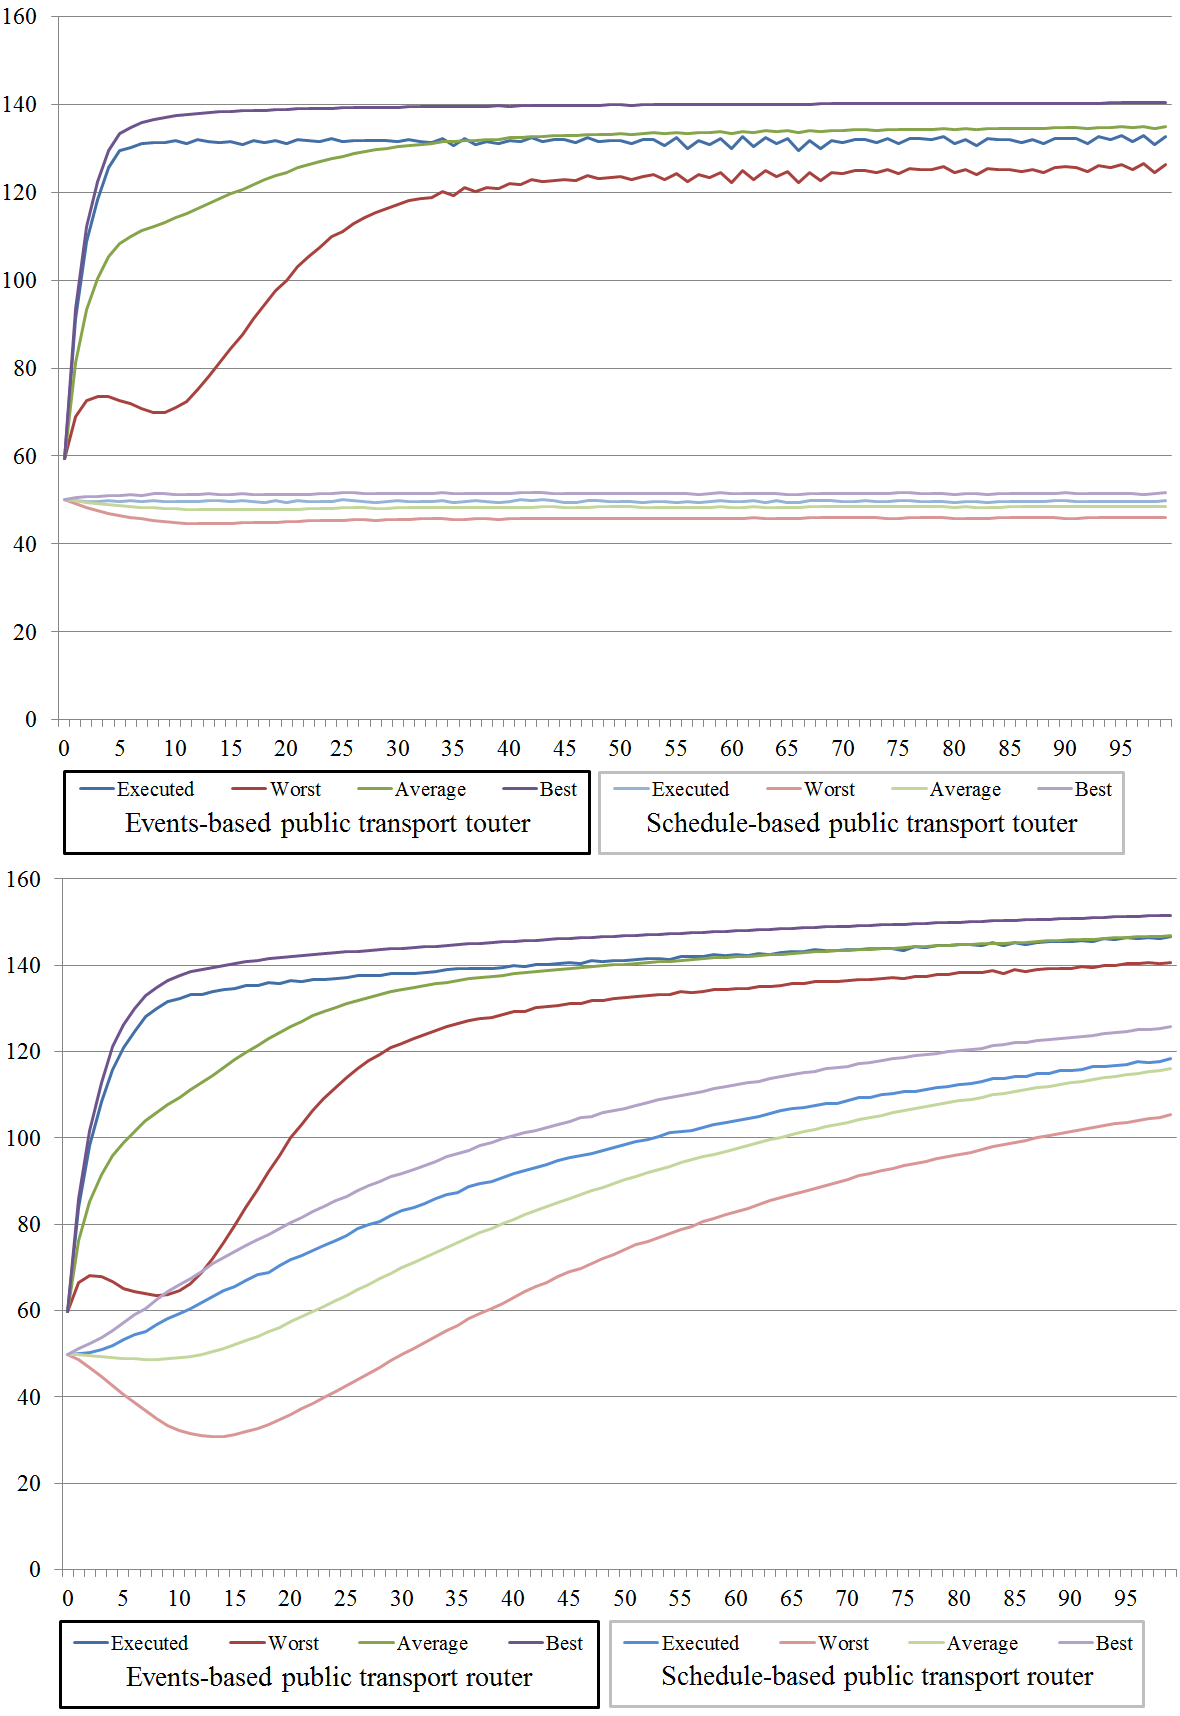
\includegraphics[width=1.0\textwidth]{extending/figures/ebr/Relaxation.png}}
{}

For the rest of the iterations, the Figure~\ref{fig:Relaxation} shows how the scores evolved. The first replanning strategy stipulated that 30\,\% of the agents were re-routed at each iteration. This evolution is shown in the first graph of the figure. Using \gls{sbptr}, agents received the same route over and over again as the start time, origin and destination did not change between iterations. Small variations in scores occurred because of the stochastic simulation nature explained above. Although scores started in the same range, using \gls{ebptr} allowed better-performing routes to be found within a very small number of iterations.

For a more realistic comparison, a second replanning strategy was tested, where just 20\,\% of the agents were re-routed and the activity start times were modified randomly within a half an hour for 10\,\% of the agents. The second graph of the figure shows how both routers managed to improve agents' plan scores. But with the \gls{ebptr}, number of iterations needed to achieve the average executed score, achieved after 100\,iterations for the \gls{sbptr} (120), was only 5. The target marginal score, as a measure of change in score over iterations, was taken arbitrarily as 0.1\,utilities per iteration, or the rate produced after 200\,iterations with the \gls{sbptr}. In contrast, this target rate was achieved after 77\,iterations with the \gls{ebptr}, a 2.6 improvement factor .

% .....................................................
\paragraph{Modeling Advantages}

Because of the links disutility function in the proposed network account for aspects like waiting times or occupancy levels and because\gls{matsim} allows for modeling heterogeneity among agents, the router could be a very powerful tool to model observed emergent behavior in public transport route choice. In Singapore, like many other crowded cities in the world, some commuters decide to travel backwards for a few stops and then transfer to a train in the opposite direction to find a seat or space in a public transport vehicle \cite{ChakirovErath_HKSTS_2011}. With the \gls{sbptr} this kind of least cost path could not be found, but with the newer proposal, this was possible. Although proportions did not match actual observations as the Singapore scenario lacked appropriate and calibrated utility parameters for traveling and waiting time under crowded conditions, Figure~\ref{fig:Backwards} showed totals of people traveling backwards from different stops in the island after 100\,iterations (see Figure~\ref{fig:Relaxation} (a)).

\createfigure
{Number of agents traveling backwards at each \protect\gls{mrt} station of the Singaporean rail system}
{Number of agents traveling backwards at each \protect\gls{mrt} station of the Singaporean rail system}
{\label{fig:Backwards}}
{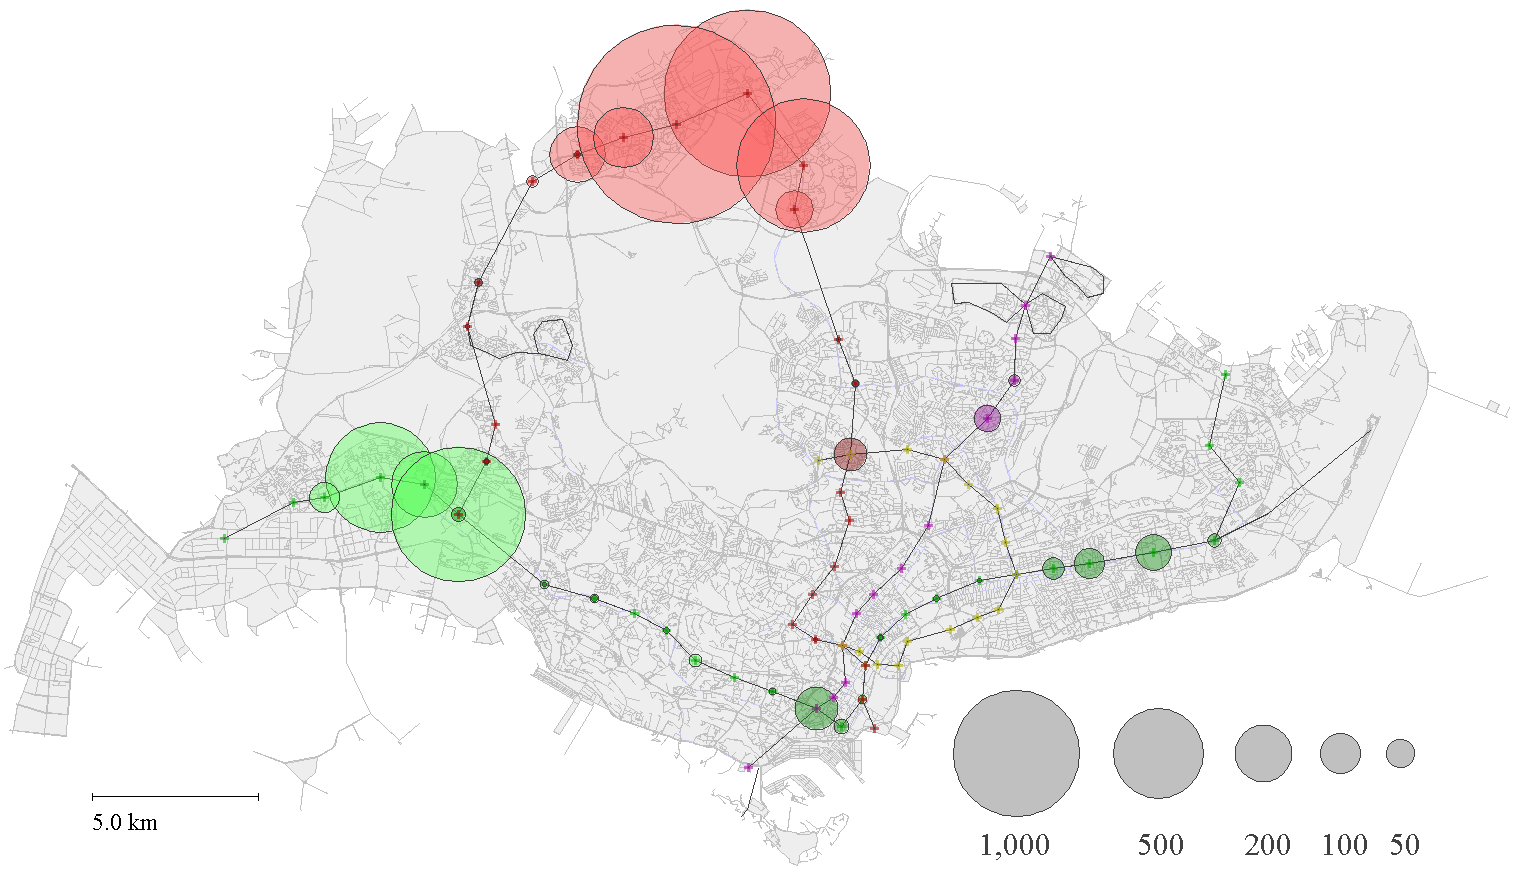
\includegraphics[width=1.0\textwidth]{extending/figures/ebr/Backwards.png}}
{}

\subsubsection{Comparing Quality Attributes With the Current Implementation}

% .....................................................
\paragraph{Computation Time}

The tests described next were executed using 12\,computational nodes, accessing 70\,\gls{gb} of shared memory, using the Singapore scenario described in Chapter~\ref{ch:singapore}. Before the first iteration, if plans were not routed, \gls{matsim} prepared every agent with an initial route. As mentioned before, the stop-stop travel times and stop-route waiting times were initially taken from the schedule. Because of its simpler network structure the \gls{ebptr} took 01:17:35 to initially route the 355\,207 users, compared with 01:28:55 needed by the \gls{sbptr}, producing a performance gain of about 12.7\,\% for this scenario. When running \gls{matsim} iterations with the \gls{ebptr}, computation times principally changed in two processes: mobility simulation (mobsim) and replanning. Figure \ref{fig:CompTimes} showed computation times measured for the first 20\,iterations of the process. Although the \gls{ebptr} needed more time in \gls{mobsim}, it continued to require considerably less time for re-routing during the replanning, due to a simpler network topology. The longer mobsim time was due to information saving in the new structures during the simulation. However, on average, the \gls{ebptr} outperformed \gls{sbptr}, per iteration, by about 3\,minutes or 11\,\%. As mentioned above, 2.6\,times more iterations were needed for the \gls{sbptr} to achieve a specific point in the relaxation process. For 77\,iterations with the \gls{ebptr}, computation amounts 35:25:43, and for 200\,iterations with the \gls{sbptr}, computation amounts 99:10:51; a 2.8 improvement factor in our experimental setting.

\createfigure
{Comparison of computation times for 20\,iterations}
{Comparison of computation times for 20\,iterations}
{\label{fig:CompTimes}}
{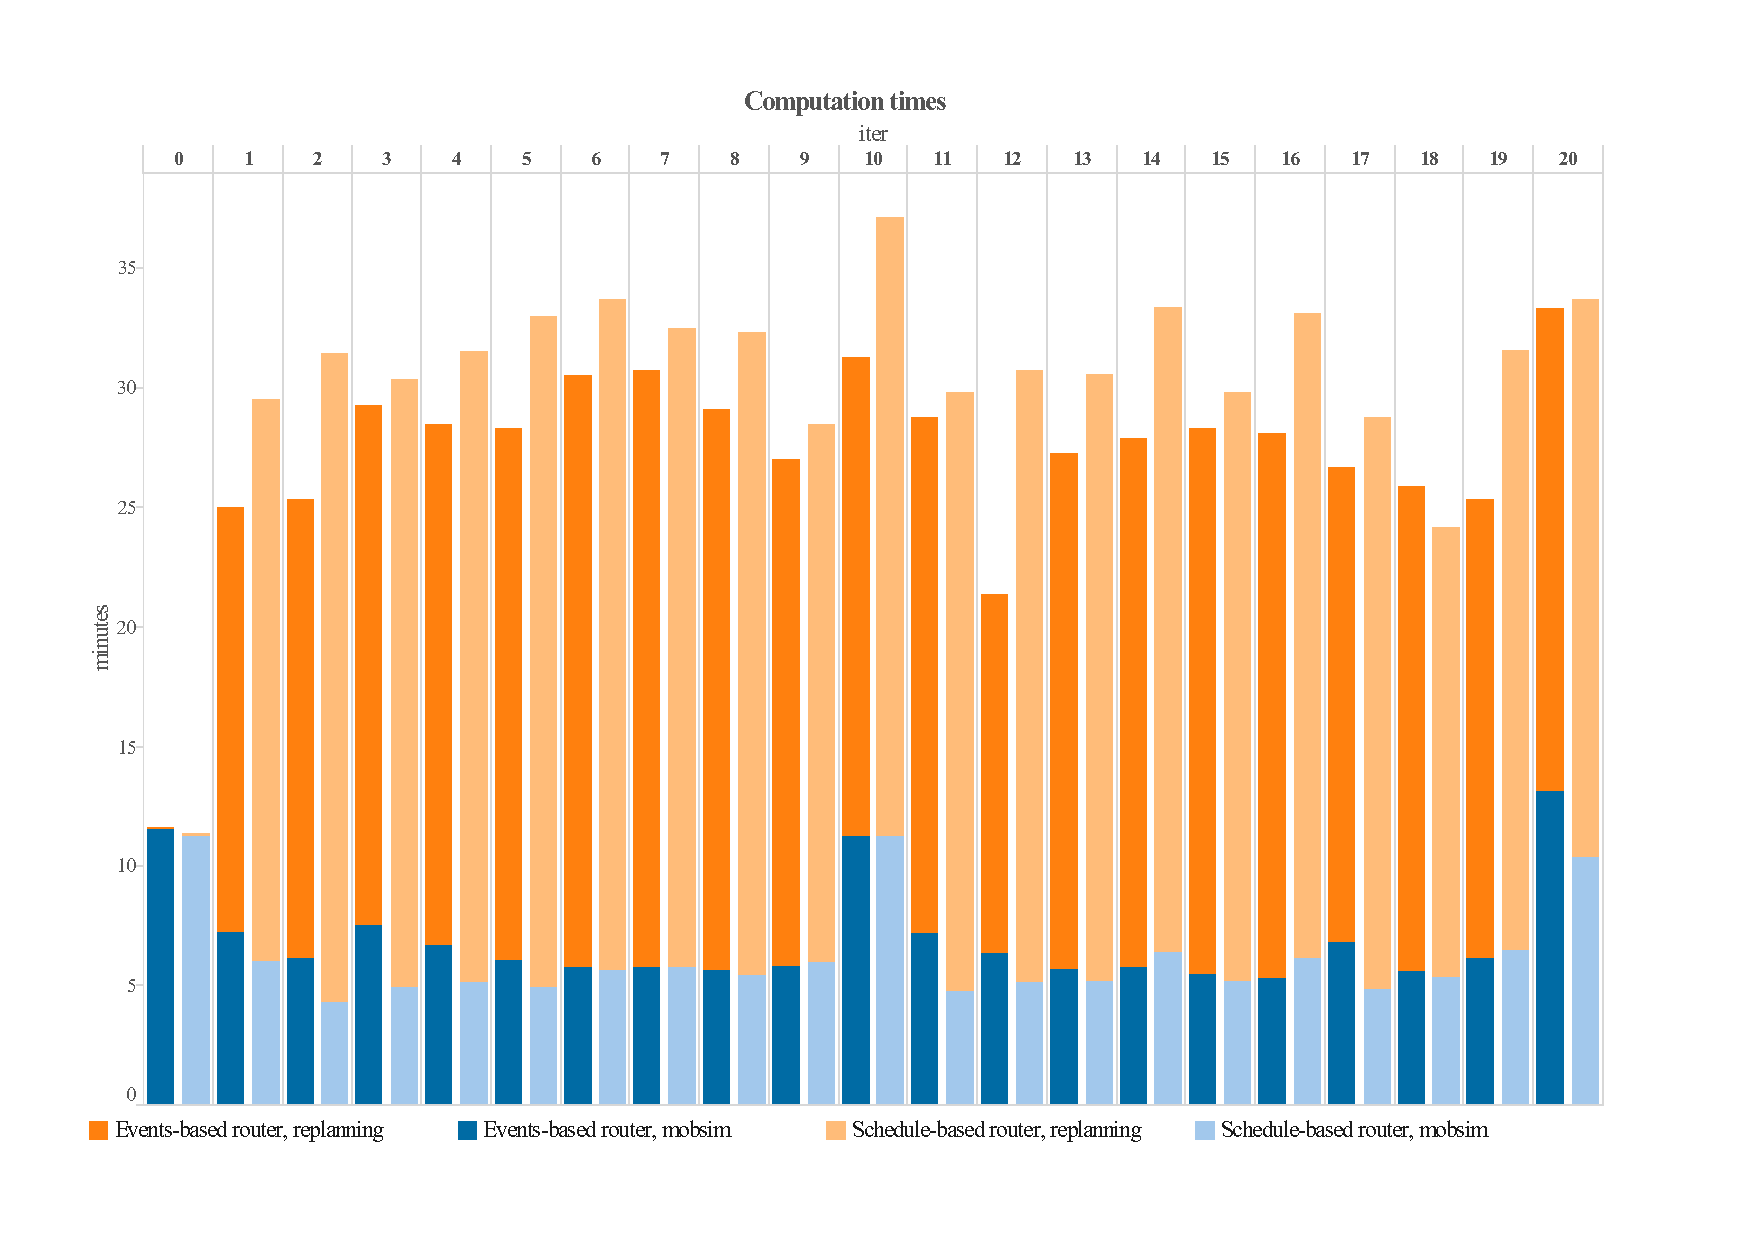
\includegraphics[width=1.0\textwidth]{extending/figures/ebr/ComputationTimes.pdf}}
{}

% .....................................................
\paragraph{Memory Consumption}

The \gls{ebptr} needed more memory than the \gls{sbptr}, because the \gls{ebptr} managed more information. The necessary extra memory was allocated to the three structures described before. Given the Singapore scenario conditions described, the extra memory was calculated as follows. One numeric value needed eight Bytes, and with a time bin of 15\,minutes, 120\,bins were needed for 30\,hours. The Stop-stop travel times structure saved two values (average and number of observations) for each time bin and each pair of consecutive stops. The number of pairs for the Singaporean public transport system was 6\,602. Thus, this structure needed approximately 12.7\,\gls{mb}. Similarly, the stop-route waiting time structure saved two values (average and number of observations) for each time bin and each pair of stop/route combinations. The number of stop/route relations for the Singaporean public transport system was 27\,156. Thus, this structure needed approximately 52.1\,\gls{mb}. Finally, the vehicle occupancy structure saved the average and number of vehicle occupancy observations for 26\,353\,route-stop relations for each of the 120\,time bins,  requiring approximately 50.7\,\gls{mb}. In total, less than 120\,\gls{mb} were needed for the three structures.

On the other hand, the size of the network where public transport routes were calculated was smaller for the \gls{ebptr}. Although, in the case of Singapore, it created 31\,939\,nodes compared with 27\,156 of the \gls{sbptr} (4\,783 new stop-nodes), the number of links is dramatically smaller. The \gls{sbptr} created 424\,070\,walking links and 26\,353\,travel links (450\,423 in total). The \gls{ebptr} created the same 26\,353\,travel links, plus 27\,156\,boarding links, plus 27\,156\,alighting links and just 4\,390\,walking links (85\,055\,links in total); less than a fifth in total. As a node needed 48\,bytes and a link 128\,bytes, the \gls{sbptr} needed roughly 46.8\,\gls{mb} more memory for links and just 229.6\,KB less for nodes. The \gls{ebptr} saved 46.5\,\gls{mb} for the network, concluding that in total the \gls{sbptr} needed 70\,\gls{mb} less memory. This quantity was negligible compared with the total memory needed for the whole simulation (more than 40\,\gls{gb}).

% ---------------------------------------------------------------------------
\subsubsection{Conclusion and Future Work} 
\label{sec:ConclusionsAndOutlook}
In this work, a new public transport router for \gls{matsim} was designed, implemented and tested. It produced more diverse routes in large scale scenarios, taking into account many complexities of urban public transport systems. On the supply side, the system simulated congestion, public transport vehicles occupancy levels, queues in public transport stops, bay sizes, and bus or train bunching. On the demand side, in addition to commonly used factors like in-vehicle time, number of transfers and walking time, the new router took disutility of additional waiting time due to congestion or overcrowded vehicles, comfort level inside public transport vehicles and preference heterogeneity among agents for all mentioned factors into account.

The utility of the new approach was tested in a large scale Singapore scenario. Using a simplified public transport only simulation, 100\,iterations of a 25\,\% scenario (355\,207 agents) with 30\,\% of the agents re-routing each iteration took just 45\,hours approximately, or about 27\,minutes per iteration, using 12\,cores and 70\,\gls{gb} of memory. The computation decreased by 11\,\% , compared to the standard \gls{matsim}. If just 20\,\% of the plans were re-routed, using 35\,cores accessing 85\,\gls{gb} of memory, the time per iteration would be reduced to less than 13\,minutes, achieving 100\,iterations in less than one day. But, most importantly, for computation time gains, we showed that the proposed events-based router was able to reach a steady state in a much smaller number of iterations.

If the proposed router works better than the original one, should it be changed? The current scheduled-based router of \gls{matsim} would still be relevant if the topology of its network were changed for the proposed one. It should also be applied to scenarios where the public transport system operates very reliably and punctually, with few cases of overcrowding. In that case, routing calculations would be as fast as the events-based router (with the new network structure), and the mobility simulation would be faster, as no information (in-vehicle time, wait time and occupancy) would be needed. In other words, it could be applied to city models where public transport users can reliably plan their trips using only a timetable.

Scrutinizing the resulting network loading, the biggest potential advantage of the proposed events-based router was its capacity to generate emergent behavior in congested public transport systems, in line with actual observations. Future research should aim at estimating the various route choice behavior parameters corresponding to the functionalities of the proposed system and calibrating the simulation. Although the values used came from a stated preference survey commissioned by the Land Transport Authority for the case of Singapore, advanced studies could, for example, be tailored to quantify preference heterogeneity. Furthermore, results from work in progress about the value of a seat in Singapore and discomfort disutility can improve prediction confidence. Finally, information from the Singapore smart card data could be used for revealed preference estimation of further behavioral parameters, like quality of a transfer described, \eg by the number of escalators, to further refine the system.
% ################################################################################################################





